\documentclass{article}
\usepackage[final]{nips_2017}
\usepackage[utf8]{inputenc} % allow utf-8 input
\usepackage[T1]{fontenc}    % use 8-bit T1 fonts
\usepackage[ngerman]{babel}
\usepackage{hyperref}       % hyperlinks
\usepackage{url}            % simple URL typesetting
\usepackage{booktabs}       % professional-quality tables
\usepackage{amsfonts}       % blackboard math symbols
\usepackage{nicefrac}       % compact symbols for 1/2, etc.
\usepackage{microtype}      % microtypography
\usepackage{placeins}
\usepackage{graphicx}
\usepackage{pgfplots}
\usepackage{biblatex} % für bibliografie
\usepackage[version=3]{acro} % akronyme

\DeclareAcronym{rbpnn}{short=RBPNN, long=radial basis probabilistic network}
\DeclareAcronym{cnn}{short=CNN, long=convolutional neural network}

\addbibresource{referenzen.bib}

\pgfplotsset{width=0.8\linewidth}
\title{Machine Learning for Computer Vision Abschlussprojekt: Rindenklassifizierung}

\author{
  Paul Walker\\
  Department of Computer Science\\
  DHBW Stuttgart\\
  \texttt{inf20045@dhbw-stuttgart.de} \\
  \And
  Tom Hofer\\
  Department of Computer Science\\
  DHBW Stuttgart\\
  \texttt{inf20173@lehre-dhbw-stuttgart.de} \\
}

\hypersetup{
  hidelinks
}

\begin{document}

\begin{center}

\includegraphics[height=0.7cm]{dhbw_logo.png}
\end{center}

\maketitle

\begin{abstract}
  % The abstract should consist of 1 paragraph describing the motivation for your paper and a high-level explanation of the methodology you used/results obtained.
  Diese Arbeit befasst sich mit der Entwicklung eines Machine Learning Modells zur Klassifikation von Rinde zu bestimmten Baumarten. 
  Das Modell könnte in der Praxis beispielsweise in einer App zur Bestimmung der Baumart anhand eines Fotos der Baumrinde eingesetzt werden. 
  Im Rahmen der Arbeit werden vier Modelle basierend auf den vortrainierten Modellen 
  InceptionV3, MobileNetV2, VGG16 und VGG19 erstellt, getestet und gegenübergestellt. 
  Für das Training der Modelle kommen ein Trainingsset mit Daten aus dem Internet, ein Entwicklungsdatensatz mit Daten aus dem Internet 
  und ein Entwicklungsdatensatz mit selbst erhobenen Daten zum Einsatz.
\end{abstract}

\section{Einleitung}
%Explain the problem and why it is important. Discuss your motivation for pursuing this
%problem. Give some background if necessary. Clearly state what the input and output
%is. Be very explicit: “The input to our algorithm is an {image, amplitude, patient age,
%rainfall measurements, grayscale video, etc.}. We then use a {SVM, neural network, linear
%regression, etc.} to output a predicted {age, stock price, cancer type, music genre, etc.}.”
%This is very important since different teams have different inputs/outputs spanning different
%application domains. Being explicit about this makes it easier for readers. If you are using
%your project for multiple classes, add a paragraph explaining which components of the
%project were used for each class.
Unser Abschlussprojekt befasst sich mit der Entwicklung eines Machine Learning Modells zur Bestimmung der Baumart anhand eines Fotos der Baumrinde. Die Rinde eignet sich sehr gut für die Bestimmung der Baumart, da diese, anders als zum Beispiel Blätter oder Früchte, unabhängig von der Jahreszeit ist. Die Eingabe für unseren Algorithmus ist also ein Bild. Zur Klassifizierung der Baumart verwenden wir ein vortrainiertes \ac{cnn}, welches wir für unseren Anwendungsfall anpassen. Die Ausgabe, beziehungsweise Vorhersage unseres Algorithmus ist die Art des Baumes, dessen Rinde auf dem Foto abgebildet ist.

In der Praxis könnte ein solches Modell zum Beispiel in einer App eingesetzt werden, 
die Baumarten bestimmen soll. 
Das Erkennen der Baumart anhand der Rinde ist ein schwieriges Problem, 
da es teilweise gro\ss e Unterschiede innerhalb einer Klasse gibt,
während zwischen Bäumen verschiedener Klassen manchmal nur sehr kleine Unterschiede erkennbar sind. 
Abbildung~\ref{problem} zeigt beispielhaft eine Kiefer, 
die sehr ähnlich zu einer Lärche aussieht 
und eine weitere Lärche, die sich von den anderen 
beiden Bäumen relativ stark unterscheidet.
Diese starken Unterschiede liegen unter anderem am Alter des Baumes.

\begin{figure}[htbp!]
  \centering
  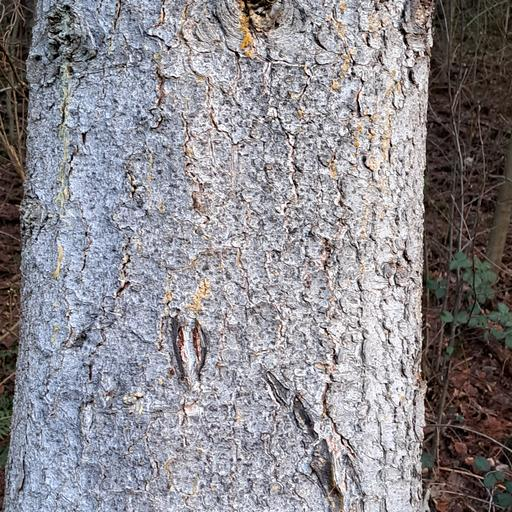
\includegraphics[width=0.32\linewidth]{examples/Kiefer.jpg}
  \includegraphics[width=0.32\linewidth]{examples/Lärche1.jpg}
  \includegraphics[width=0.32\linewidth]{examples/Lärche2.jpg}\\
  Kiefer \hspace{100px} Lärche \hspace{100px} Lärche
  \caption{Schwierigkeit des Problems}
  \label{problem}
\end{figure}

\section{Stand der Technik}
%[Optional and seen as extension] You can find existing papers, and see how they are similar to and differ
%from your work. In your opinion, which approaches were clever/good? What is the stateof-the-art?
%Do most people perform the task by hand? This includes previous attempts by others at your problem,
%previous technical methods, or previous learning algorithms. Google Scholar is very useful
%for this: https://scholar.google.com/ (you can click “cite” and it generates MLA, APA,
%BibTeX, etc.)
Die Rindenklassifikation ist kein neues Problem und es wurden bereits Ansätze sowohl mit klassischer Computer Vision~\cite{bark_texture}, als auch mit Hilfe von Deep Learning entwickelt~\cite{1_CNN_bark}.
In einigen Ansätzen wird ein radial \ac{rbpnn} anstatt einem \ac{cnn} verwendet~\cite{rbpnn_bark}.
Viele Paper, in denen ein \ac{cnn} genutzt wird, verwenden ein vortrainiertes \ac{cnn}~\cite{1_CNN_bark},
dass dann nur noch auf das Problem spezialisiert wird.
Dieser Ansatz wird auch in dieser Arbeit verfolgt.

\section{Daten und Features}
%Describe your dataset: how many training/validation/test examples do you have? Is there
%any preprocessing you did? What about normalization or data augmentation? What is the
%resolution of your images? How is your time-series data discretized? Include a citation on
%where you obtained your dataset from. Depending on available space, show some examples
%from your dataset. You should also talk about the features you used. If you extracted
%features using Fourier transforms, word2vec, PCA,
%ICA, etc. make sure to talk about it. Try to include examples of your data in the report
%(e.g. include an image, show a waveform, etc.).

Wir nutzen 21491 Bilder aus dem Internet bestehend aus 8 verschiedenen Klassen.
Die Daten stammen aus dem BARK-KR~\cite{2_BARK-KR} Datenset, 
dem Tree Species Dataset~\cite{3_Tree_species} 
und dem BarkNet~1.0~\cite{4_barkNet} Datenset. 
Einige Beispiele dieser Daten sind in Abbildung~\ref{train} abgebildet. 
Neben diesen Daten nutzen wir auch 333 selbst gelabelte Bilder bestehend aus denselben 8 Klassen.
Einige Beispiele sind in Abbildung~\ref{validation} abgebildet.

Diese Daten werden aufgeteilt in ein Trainingsset bestehend aus 21169 Bildern aus den Internetdaten
und zwei verschiedene Entwicklungsdatensätze,
einem bestehend aus 322 Bildern aus den Internetdaten (dev-set 1) 
und einem bestehend aus den 333 selbst gelabelten Bildern (dev-set 2)
Ein Testset haben wir nicht. 
Wir können also keine genaue Aussage über die tatsächliche Feldperformance unseres Modells treffen. 
Es werden zwei verschiedene Entwicklungsdatensätze genutzt, 
da die Daten aus dem Internet und die selbst gelabelten Daten stark verschieden sind.
Das sorgt dafür, dass die Genauigkeit des Models auf den selbst gelabelten Daten durchgängig schlecht ist.
Der Entwicklungsdatensatz aus dem Internet vereinfacht die Entwicklung,
da auf diesem das Model eine höhere Genauigkeit hat und Overfitting damit schneller erkennbar ist.

Alle Bilder werden auf eine Grö\ss e von 512*512 Pixeln gebracht. Um Verzerrungen zu vermeiden werden die Grafiken zunächst durch Zuschneiden auf das richtige Seitenverhältnis gebracht. In unseren Datensätzen haben wir acht Klassen, beziehungsweise acht Baumarten. 
Die Datensätze aus dem Internet bieten zwar noch weitaus mehr Klassen, allerdings sind für diese keine selbst gelabelten Daten vorhanden. 
Zusätzlich mussten die Labels der Daten aus dem Internet angepasst werden,
da diese die Bäume noch in genaue Unterarten einteilen.
Für diesen Rinden-klassifikator ist allerdings nur die Überart relevant. 
So wird beispielsweise das Label "Orientalische Wei\ss -Eiche - Quercus aliena" in unserem Datensatz einfach als Oak, also Eiche, gelabelt. 
Die vertretenen Baumarten sind Esche, Buche, Birke, Tanne, Lärche, Eiche, Kiefer und Fichte.

\begin{figure}[h!]
  \centering
  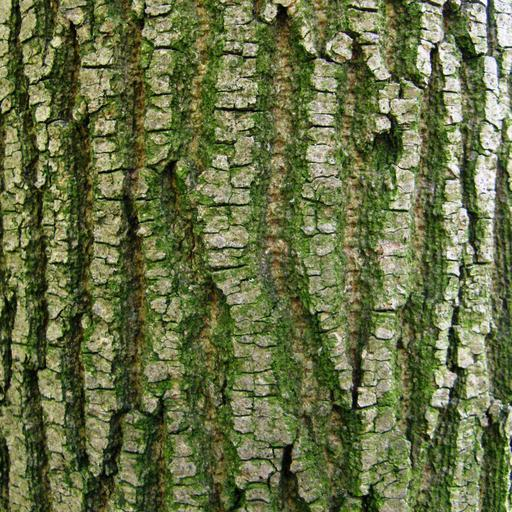
\includegraphics[width=0.24\linewidth]{examples/train/Ash}
  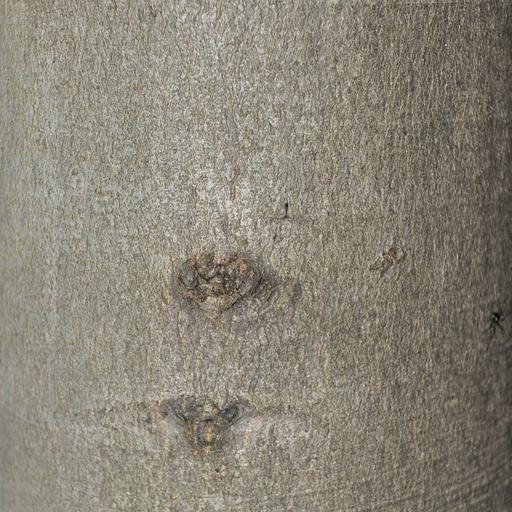
\includegraphics[width=0.24\linewidth]{examples/train/Beech}
  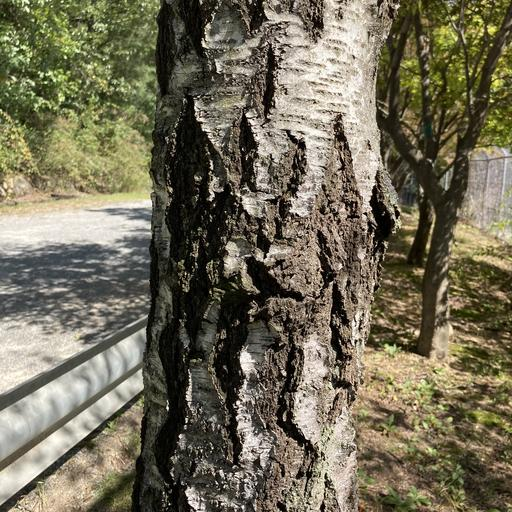
\includegraphics[width=0.24\linewidth]{examples/train/Birch}
  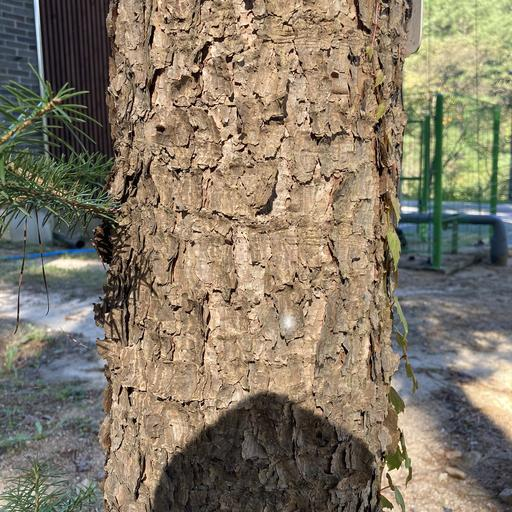
\includegraphics[width=0.24\linewidth]{examples/train/Fir}
  Esche \hspace{70pt} Buche \hspace{70pt} Birke \hspace{70pt} Tanne\\
  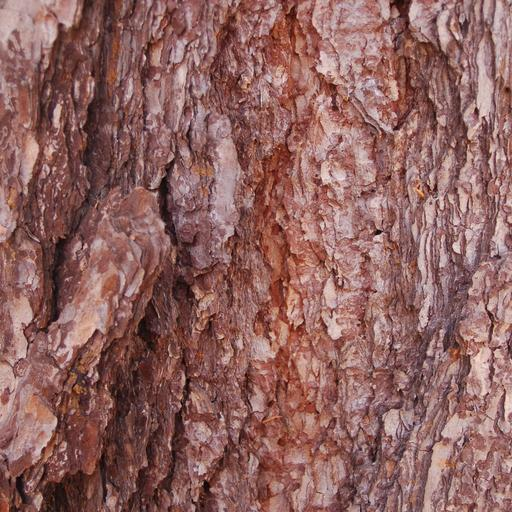
\includegraphics[width=0.24\linewidth]{examples/train/Larch}
  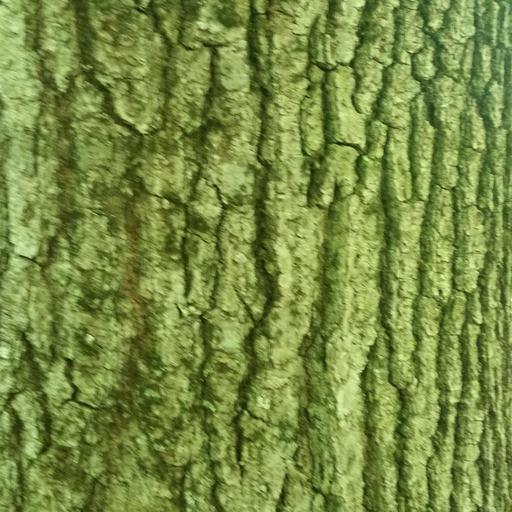
\includegraphics[width=0.24\linewidth]{examples/train/Oak}
  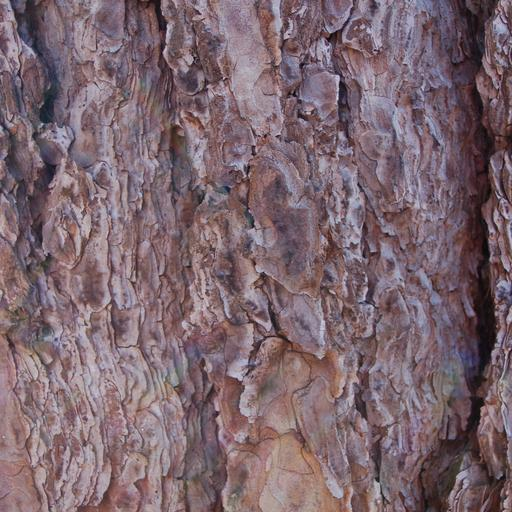
\includegraphics[width=0.24\linewidth]{examples/train/Pine}
  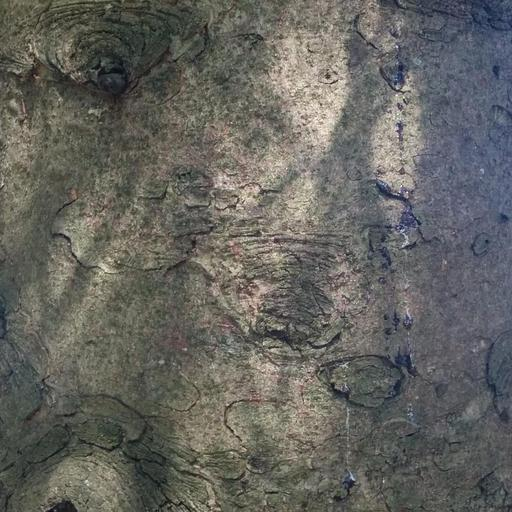
\includegraphics[width=0.24\linewidth]{examples/train/Spruce}
  Lärche \hspace{70pt} Eiche \hspace{70pt} Kiefer \hspace{70pt} Fichte\\
  \caption{Beispiele aus den Trainingsdaten}
  \label{train}
\end{figure}

\begin{figure}[h!]
  \centering
  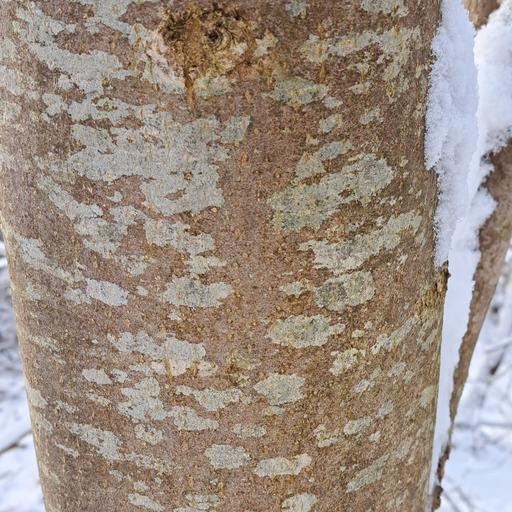
\includegraphics[width=0.24\linewidth]{examples/validation/Ash}
  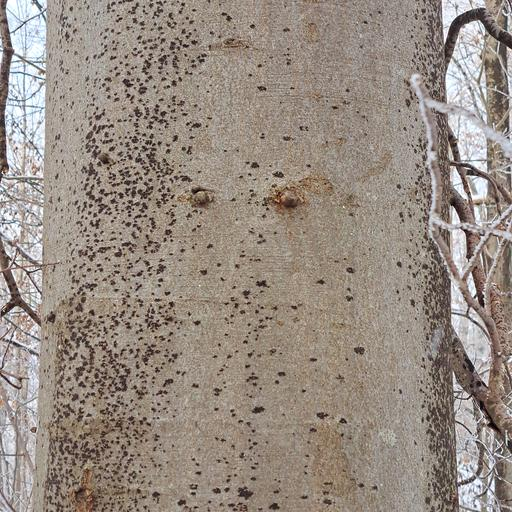
\includegraphics[width=0.24\linewidth]{examples/validation/Beech}
  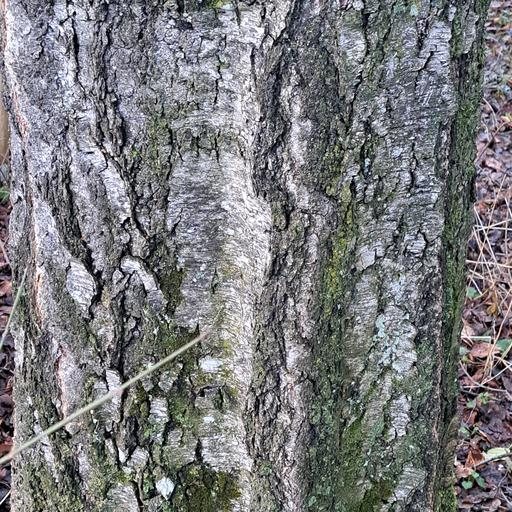
\includegraphics[width=0.24\linewidth]{examples/validation/Birch}
  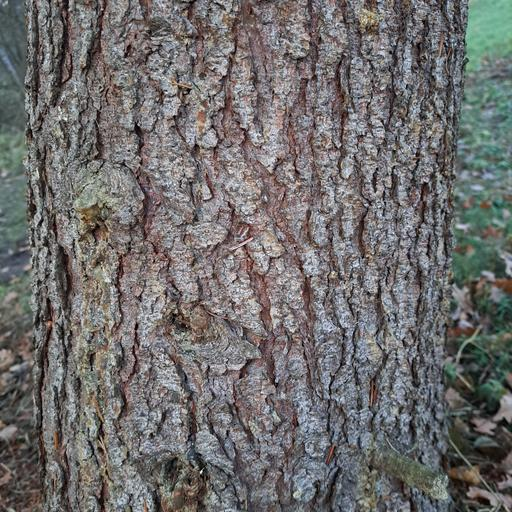
\includegraphics[width=0.24\linewidth]{examples/validation/Fir}
  Esche \hspace{70pt} Buche \hspace{70pt} Birke \hspace{70pt} Tanne\\
  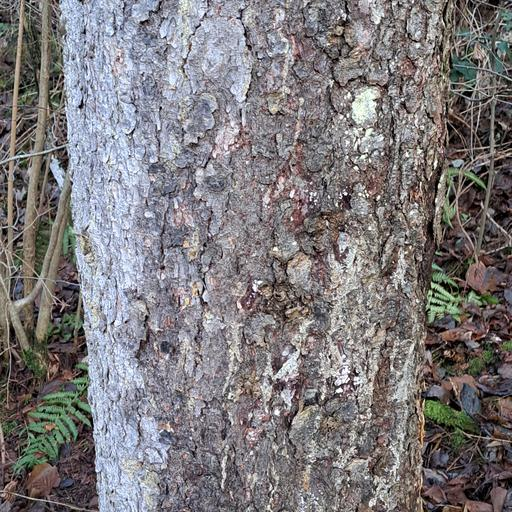
\includegraphics[width=0.24\linewidth]{examples/validation/Larch}
  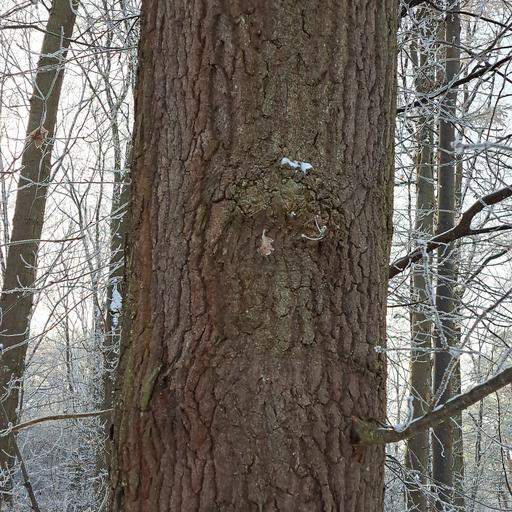
\includegraphics[width=0.24\linewidth]{examples/validation/Oak}
  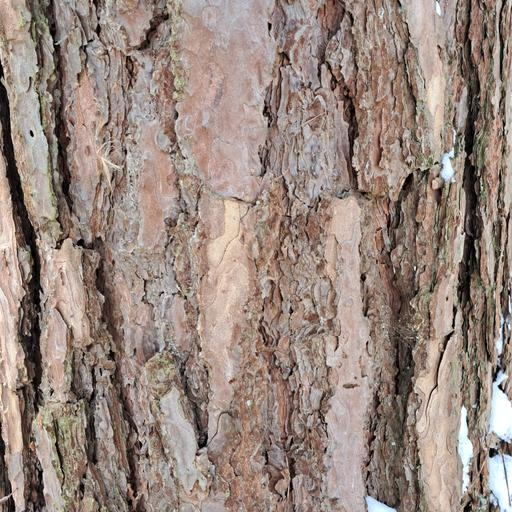
\includegraphics[width=0.24\linewidth]{examples/validation/Pine}
  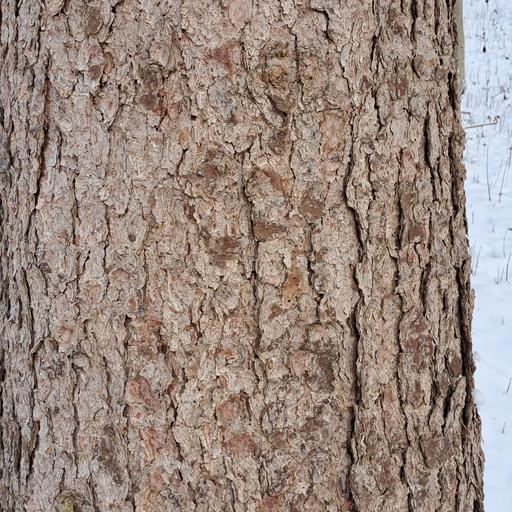
\includegraphics[width=0.24\linewidth]{examples/validation/Spruce}
  Lärche \hspace{70pt} Eiche \hspace{70pt} Kiefer \hspace{70pt} Fichte\\
  \caption{Baspiele aus dem Validationset}
  \label{validation}
\end{figure}

\section{Methoden}
%Describe your learning algorithms, proposed algorithm(s), or theoretical proof(s). Make
%sure to include relevant mathematical notation. For example, you can include the loss function you are using. It is okay to use formulas from the lectures (online or in-class). For each algorithm, give a short description 
%of how it works. Again, we are looking for your understanding of how these deep
%learning algorithms work. Although the teaching staff probably know the algorithms, future
%readers may not. Additionally, if you are
%using a niche or cutting-edge algorithm (anything else not covered in the class), you may want to explain your algorithm using 1/2
%paragraphs. Note: Theory/algorithms projects may have an appendix showing extended
%proofs (see Appendix section below).

Zur Erstellung unseres Modells verwenden wir Transfer learning. Das bedeutet wir verwenden ein bereits für Bilddaten Trainiertes \ac{cnn} aus dem Internet und passen dieses auf unseren Anwendungsfall an. 
Die Anpassung erfolgt in den Ersten und letzten Schichten des Modells. 

Die erste Schicht ist die Eingabeschicht, die ein Bild mit 512*512 Pixeln und drei Kanälen annimmt. 
Dazu wird eine Schicht hinzugefügt, die die Bilder von einem Wertebereich von 0 bis 255 auf einen Wertebereich von 0 bis 1 transformiert.
Für die Ausgabe des Modells werden vier Schichten am Ende hinzugefügt. 
Zunächst erfolgt ein zweidimensionales global average pooling,
gefolgt von einer flatten und dense Schicht. 
Die dense Schicht verwendet eine Relu als Aktivierungsfunktion. 
In der letzten Schicht wird die Ausgabe des Modells nochmal auf die Anzahl an Klassen, 
also in unserem Fall acht, heruntergebrochen. 
Die Letzte Schicht ist ein Softmax-Layer. 
Diese Schichten, die am Ende zu dem Model hinzugefügt wurden sind in der Abbildung~\ref{VGG16} rot markiert,
diejenigen, die am Anfang des Models hinzugefügt wurden sind in der Abbildung~\ref{VGG16} grün markiert.
Um unser Model zu trainieren, verwenden wir sparse categorial crossentropy loss.

Die Abbildung zeigt die in diesem Paper gemachten Ergänzungen an einem VGG16 Model.
Neben diesem Model wurden diese Ergänzungen noch an einem InceptionV3 model,
einem MobileNetV2 model und einem VGG19 model gemacht und die Ergebnisse verglichen.



\begin{figure}[htbp!]
  \centering
  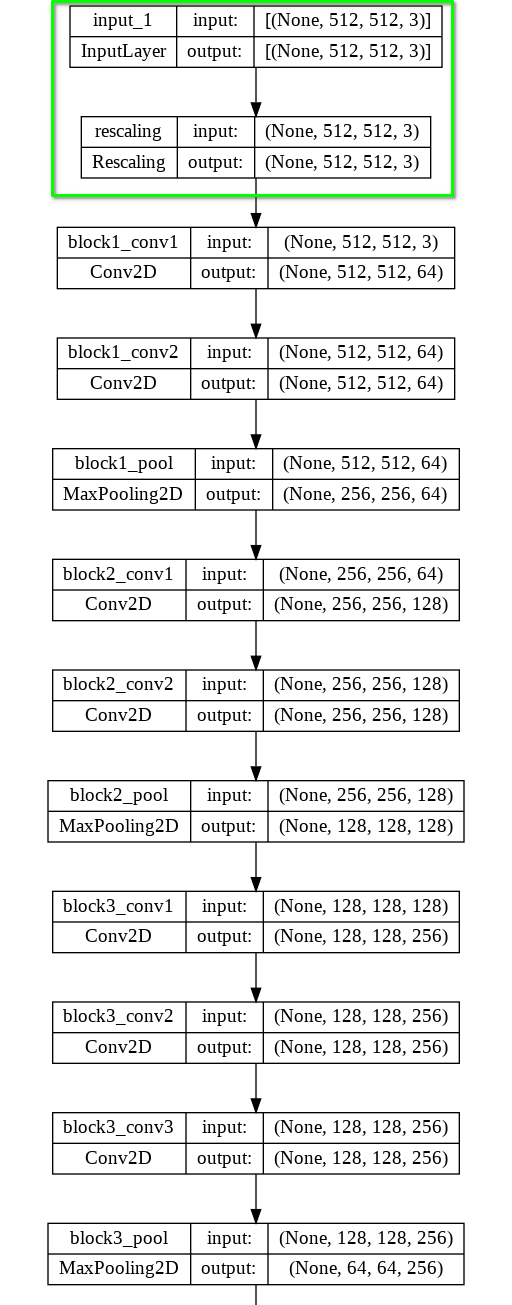
\includegraphics[width=0.4\linewidth]{VGG16_top}
  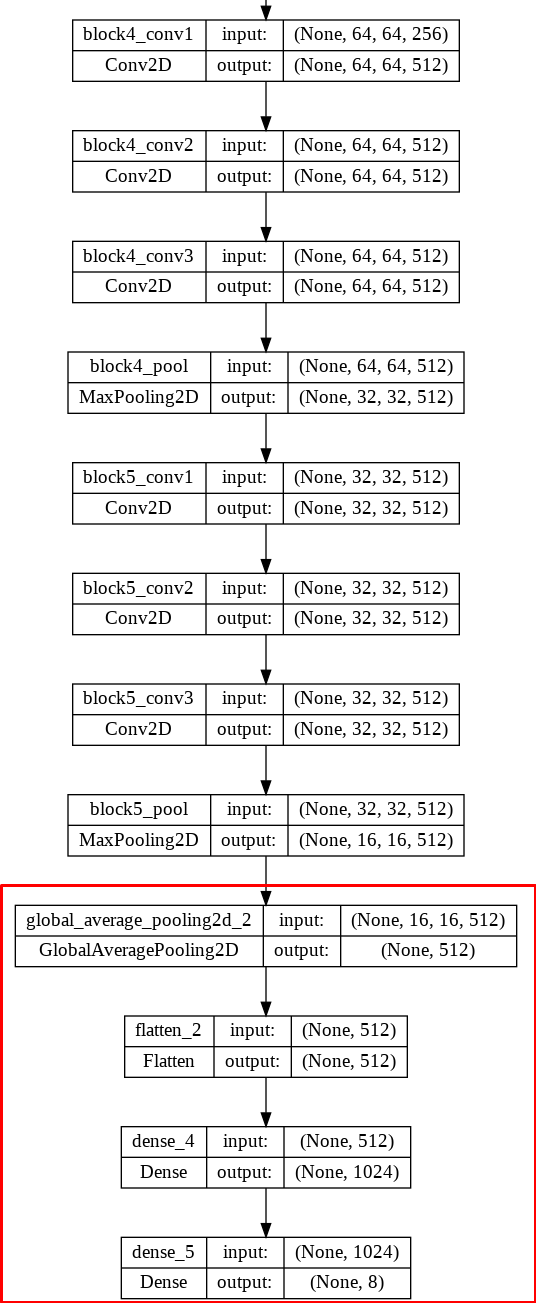
\includegraphics[width=0.4\linewidth]{VGG16_bottom}
  \caption{Darstellung des auf VGG16 basierenden Modells}
  \label{VGG16}
\end{figure}

\FloatBarrier

\section{Experimente/Ergebnisse/Diskussion}
%You should also give details about what (hyper)parameters you chose (e.g. why did you
%use X learning rate for gradient descent, what was your mini-batch size and why) and how
%you chose them. What your primary metrics are: accuracy, precision,
%AUC, etc. Provide equations for the metrics if necessary. For results, you want to have a
%mixture of tables and plots. If you are solving a classification problem, can include a
%confusion matrix. Include performance metrics such as precision,
%recall, and accuracy. For regression problems, state the average error. You should have
%both quantitative and qualitative results. To reiterate, you must have both quantitative
%and qualitative results! If it applies: include visualizations of results, heatmaps,
%examples of where your algorithm failed and a discussion of why certain algorithms failed
%or succeeded. In addition, explain whether you think you have overfit to your training set
%and what, if anything, you did to mitigate that. Make sure to discuss the figures/tables in
%your main text throughout this section. Your plots should include legends, axis labels, and
%have font sizes that are legible when printed.

Wir haben verschiedene vortrainierte Basismodelle ausprobiert und deren Performance gegenübergestellt. 
Die betrachteten vortrainierten Modelle sind InceptionV3, MobileNetV2, VGG16 und VGG19. 
Die Ergebnisse der Gegenüberstellung sind in Abbildung~\ref{vergleich} dargestellt. 
Die höchste Performance erzielt MobileNetV2 mit einer Trefferate von 52,85\% auf dem Entwicklungsdatensatz dev-set 2 mit unseren selbst gelabelten Daten. 
Bei acht Klassen würde man mit zufälliger Auswahl auf eine Trefferate von 12,5\% kommen, 
das Modell ist also deutlich besser als zufällige Auswahl. 
Da alle Modelle jedoch auf unseren selbst gelabelten Daten eine sehr viel geringere Trefferchance haben als beim Taining,
ist es wichtig auch den Entwicklungsdatensatz dev-set 1 mit den Daten aus dem Internet zu betrachten.
Auf diesen Daten weisen die Modelle eine ähnliche Trefferrate wie beim Training auf. 
Unsere Modelle können also nicht gut von den Trainingsdaten auf die selbst gelabelten Daten generalisieren. 
Ursache dafür können regional verschiedenen Unterarten sein 
oder auch die verschiedenen Licht- und Wetterverhältnisse, bei denen die Bilder gemacht wurden.
Die selbst gelabelten Daten wurden im Winter bei Schnee fotografiert, 
während die meisten der Daten aus dem Internet bei guten Lichtverhältnissen
und nicht mit Schnee im Hintergrund fotografiert wurden.
Um ein besseres Ergebnis zu erzielen, 
müssten mehr regionale Daten bei verschiedenen 
Licht- und Wetterverhältnissen erhoben werden, 
die dem Trainingsset hinzugefügt werden.

Um die Performance weiter zu verbessern wurde das beste Model (MobileNetV2) ausgewählt
und auf diesem ein Fine-Tuning schritt durchgeführt.
Dafür werden die unteren 15 Layer des Models mit einer niedrigen Learningrate nachtrainiert.
Das sorgt für eine Performanceverbesserung auf den Trainingsdaten und den Entwicklungsdaten aus dem Internet (dev-set 1),
die Performance auf den selbst gelabelten Entwicklungsdaten sinkt allerdings etwas (siehe Abbildung~\ref{fine_tuning}).

\begin{figure}[h!]
  \centering
  \begin{tikzpicture}
    \begin{axis}[
      ybar,
      enlargelimits=0.25,
      legend style={at={(0.5,-0.13)},
        anchor=north,legend columns=-1},
      ylabel={accuracy in \%},
      symbolic x coords={InceptionV3,MobileNetV2,VGG16,VGG19},
      xtick=data,
      nodes near coords,
      nodes near coords style={font=\small, rotate=90, anchor=west}
      %nodes near coords align={vertical}
      ]
      \addplot % training
      coordinates {(InceptionV3,85.31) (MobileNetV2,90.55) (VGG16,76.02) (VGG19,69.61)};
      \addplot % validation internet
      coordinates {(InceptionV3,86.34) (MobileNetV2,88.82) (VGG16,75.16) (VGG19,70.50)};
      \addplot % validation self labeled
      coordinates {(InceptionV3,45.65) (MobileNetV2,52.85) (VGG16,28.83) (VGG19,24.62)};
      \legend{training,dev set 1 (internet), dev-set 2 (self labeled)}
    \end{axis}
  \end{tikzpicture}
  \caption{Vergleich der verschiedenen Modelle}
  \label{vergleich}
\end{figure}

\begin{figure}[h!]
  \centering
  \begin{tikzpicture}
    \begin{axis}[
      ybar,
      enlargelimits=0.25,
      legend style={at={(0.5,-0.13)},
        anchor=north,legend columns=-1},
      ylabel={accuracy in \%},
      symbolic x coords={MobileNetV2 (fine tuned)},
      xtick=data,
      nodes near coords,
      nodes near coords style={font=\small, rotate=90, anchor=west}
      %nodes near coords align={vertical}
      ]
      \addplot % training
      coordinates {(MobileNetV2 (fine tuned),93.98)};
      \addplot % validation internet
      coordinates {(MobileNetV2 (fine tuned),92.50)};
      \addplot % validation self labeled
      coordinates {(MobileNetV2 (fine tuned),48.35)};
      \legend{training,dev set 1 (internet), dev-set 2 (self labeled)}
    \end{axis}
  \end{tikzpicture}
  \caption{fine tuned MobileNetV2}
  \label{fine_tuning}
\end{figure}

\FloatBarrier

\section{Fazit und Ausblick}
%Summarize your report and reiterate key points. Which algorithms were the highestperforming?
%Why do you think that some algorithms worked better than others? For
%future work, if you had more time, more team members, or more computational resources,
%what would you explore?

In dieser Arbeit wurden vier neuronale Netze mittels Transfer Learning aus vier vortrainierten Modellen erstellt. 
Diese wurden mit Bildern von Rinde aus dem Internet trainiert, 
mit dem Ziel der Klassifikation zu einer von acht Baumarten. 
Zusätzlich wurden händisch Daten erhoben und gelabelt, die ein Entwicklungsdatensatz (dev-set 2) bildeten. 
Ein zweiter Entwicklungsdatensatz (dev-set 1) wurde aus einem Teil der Daten aus dem Internet erstellt. 
Die vier entwickelten Modelle wurden nach ihrer Treffwahrscheinlichkeit gegenübergestellt. 
Außerdem wurde eine schlechte Generalisierungsfähigkeit der Modelle von den externen auf die selbst erstellten Daten festgestellt.
Da die Performance auf dem Entwicklungsdatensatz aus dem Internet (dev-set 1) 
sehr nahe an der Performance auf den Trainingsdaten liegt, 
kann davon ausgegangen werden, 
dass bei einem Training des Modells mit regionalen Daten 
eine ähnlich hohe Performance erreicht werden kann.

\section*{Referenzen}
%This section should include citations for: (1) Any papers mentioned in the related work
%section. (2) Papers describing algorithms that you used which were not covered in class.
%(3) Code or libraries you downloaded and used. This includes libraries such as scikit-learn, Tensorflow, Pytorch, Keras etc. Acceptable formats include: MLA, APA, IEEE. If you
%do not use one of these formats, each reference entry must include the following (preferably
%in this order): author(s), title, conference/journal, publisher, year. If you are using TeX,
%you can use any bibliography format which includes the items mentioned above. We are excluding
%the references section from the page limit to encourage students to perform a thorough
%literature review/related work section without being space-penalized if they include more
%references. Any choice of citation style is acceptable
%as long as you are consistent.
\subsection*{Verwendete Softwarebibliotheken}
\begin{itemize}
\item Pillow-SIMD
\item google.colab (drive)
\item Tensorflow
\item os
\item Keras
\item matplotlib
\end{itemize}

\medskip
\small

\printbibliography[heading=none]

\end{document}